\documentclass[11pt,a4paper]{article}

\usepackage[utf8x]{inputenc}   % omogoča uporabo slovenskih črk kodiranih v formatu UTF-8
\usepackage[slovene]{babel}    % naloži, med drugim, slovenske delilne vzorce

\usepackage[hyphens]{url}
\usepackage{hyperref}
\usepackage[pdftex]{graphicx}
\usepackage{float}


\title{Seminarska naloga: Seam Carving}
\author{Amon Stopinšek\\
63150273\\
\ \\
Vzporedni in porazdeljeni sistemi in algoritmi \\
Fakulteta za računalništvo in informatiko Univerze v Ljubljani
\date{\today}         
}



\begin{document}
\maketitle

\section{Opis problema}
Rezanje šivov je algoritem za spreminjanje velikosti slik. Algoritem 
upošteva vsebino slike tako, da pride pri spreminjanju velikosti do
čim manjšega popačenja. V vsakem koraku se odstrani šiv (povezano
zaporedje pikslov od vrha do dna ali od levega do desnega roba slike)
z najmanj pomembno vsebino.


Algoritem:
\begin{enumerate}
\item Izračunaj energijo vsakega piskla na sliki (npr. z uporabo sobelovega filtra za detekcijo robov).
\item Poišči najmanjši šiv (npr. izračunaj vse šive z dinamičnim programiranjem in poišči najmanjši šiv).
\item Odstani šiv.
\item Ponovi celoten postopek dokler slika ni želene velikosti.
\end{enumerate}

\section{Opis arhitekture in pristopa k reševanju}
Implementirali smo dve verziji algoritma - serijsko in paralelno.

V obeh implementacijah smo za računanje energij uporabili
sobelov filter, za iskanje najmanjšega šiva pa smo implementirali
algoritem s pomočjo dinamičnega programiranja.

Posebnosti obeh implementacij so opisane v sekciji \ref{serial} in \ref{paralel}.

\subsection{Splošne značilnosti}
Za delo s slikami smo uporabili knjižico pgm. Knjižica podpira
branje in shranjevanje slik v formatu pgm.



Za računanje energij smo uporabili sobelov filter.

Iskanje najmanjšega šiva smo implementirali s pomočjo dinamičnega
programiranja. V vsaki vrstici za vsak piksel izračunamo skupno 
energijo najmanjšega možnega šiva do te vrstice. Po tem postopku 
v zadnji vrstici dobimo vrednosti najmanjših šivov. Izmed teh
poiščemo najmanjši šiv.

\subsection{Serijski algoritem}
\label{serial}
\subsubsection{Iskanje in odstranjevanje najmanjšega šiva}

Ob rekonstrukciji najmanjšega šiva sproti kopiramo piksle
za novo sliko.

\subsection{Paralelni algoritem}
\label{paralel}

\subsubsection{Sobelov filter}
Za izračun sobelovega filtra poženemo toliko niti kolikor je
pikslov na sliki. Vrednosti zunaj slike imajo vrednost 0.

\subsubsection{Iskanje najmanjšega šiva}
Zaradi potrebe po sinhronizaciji med nitmi poženemo samo en
workgroup. Odvisno od velikosti slike vsaka nit za vsako
vrstico v sliki izračuna vrednosti za nič ali več pikslov.

Najmanjši šiv nato poiščemo s pomočjo redukcije.

Rezultat iskanja je tabela z indeksi šiva.

\subsubsection{Odstranjevanje šiva}
Za odstranjevanje šiva poženemo toliko niti kolikor je število
pikslov na originalni sliki. Vsaka nit, katere indeks ni čez
širino nove slike skopira piksel iz originalne slike na
ustrezno mesto na novi sliki.

\pagebreak

\section{Rezultati}
Obe implementaciji smo testirali na 7 različnih slikah.

\begin{table}[htbp]
\begin{center}
\begin{tabular}{|l|c|c|}
	\hline
		& serijski & paralelni  \\
	\hline
	število meritev & 245 & 286\\
	\hline
	povprečna pohitritev & 0.6321 & 1.709\\
    \hline
    mediana pohitritev & 0.5304 & 1.885\\
    \hline
     standardna deviacija pohitritev & 0.2341 & 0.4072\\
    \hline
\end{tabular}
\end{center}

\caption{Povprečni rezultati}
\label{table:ta}
\end{table}


Na sliki~\ref{pic1} in ~\ref{pic2} sta prikazana
grafa pohitritve paralelnega algoritma v primerjavi
s serijskim v odvisnosti od velikosti slike.


Na manjši sliki se je za hitrejšo izkazala serijska 
implementacija, na vseh preostalih slikah pa je bila
hitrejša paralelna verzija. 



\subsection{Slika: cubes}

\begin{itemize}
\item Velikost slike: 478px × 478px
\item Število iteracij: 400
\end{itemize}

\begin{table}[htbp]
\begin{center}
\begin{tabular}{|l|c|c|}
	\hline
		& serijski & paralelni  \\
	\hline
	število meritev & 50 & 50 \\
	\hline
	povprečni čas izvajanja & 0.6559  & 0.752\\
    \hline
    mediana &  0.654  & 0.7497\\
    \hline
    	standardna deviacija & 0.003456 & 0.01374  \\
    \hline
    pohitritev & 1.1465 & 0.8722 \\
    \hline
\end{tabular}
\end{center}

\caption{Rezultati za sliko cubes}
\label{table:ta}
\end{table}


\subsection{Slika: tower}

\begin{itemize}
\item Velikost slike: 1280px × 868px
\item Število iteracij: 400
\end{itemize}

\begin{table}[htbp]
\begin{center}
\begin{tabular}{|l|c|c|}
	\hline
		& serijski & paralelni  \\
	\hline
	število meritev & 50 & 50 \\
	\hline
	povprečni čas izvajanja & 4.597 & 3.079\\
    \hline
    mediana & 4.596  & 3.07\\
    \hline
    	standardna deviacija & 0.007714  & 0.06314\\
    \hline
    pohitritev & 0.6698 & 1.4930\\
    \hline
\end{tabular}
\end{center}

\caption{Rezultati za sliko tower}
\label{table:ta}
\end{table}

\pagebreak

\subsection{Slika: bike}

\begin{itemize}
\item Velikost slike: 2592px × 1456px
\item Število iteracij: 400
\end{itemize}

\begin{table}[htbp]
\begin{center}
\begin{tabular}{|l|c|c|}
	\hline
		& serijski & paralelni  \\
	\hline
	število meritev & 50 & 50\\
	\hline
	povprečni čas izvajanja & 17.11  & 9.076\\
    \hline
    mediana & 17.1  & 8.952\\
    \hline
    	standardna deviacija & 0.02976  & 0.2548 \\
    \hline
    pohitritev & 0.5304 & 1.8852 \\
    \hline
\end{tabular}
\end{center}

\caption{Rezultati za sliko bike}
\label{table:ta}
\end{table}

\subsection{Slika: wires}


\begin{itemize}
\item Velikost slike: 2592px × 1728px
\item Število iteracij: 400
\end{itemize}

\begin{table}[htbp]
\begin{center}
\begin{tabular}{|l|c|c|}
	\hline
		& serijski & paralelni  \\
	\hline
	število meritev & 50 & 50\\
	\hline
	povprečni čas izvajanja & 20.31  & 10.4 \\
    \hline
    mediana & 20.3  & 10.39\\
    \hline
    	standardna deviacija & 0.04101  & 0.05947\\
    \hline
    pohitritev & 0.5121 & 1.9529\\
    \hline
\end{tabular}
\end{center}

\caption{Rezultati za sliko wires}
\label{table:ta}
\end{table}

\subsection{Slika: texture}

\begin{itemize}
\item Velikost slike: 5160px × 3870px
\item Število iteracij: 400
\end{itemize}

\begin{table}[htbp]
\begin{center}
\begin{tabular}{|l|c|c|}
	\hline
		& serijski & paralelni  \\
	\hline
	število meritev & 50 & 25 \\
	\hline
	povprečni čas izvajanja & 123.4  & 67.85 \\
    \hline
    mediana  & 123.7 & 68.52\\
    \hline
    	standardna deviacija & 1.602  & 5.775\\
    \hline
    pohitritev & 0.5498 &  1.8187\\
    \hline
\end{tabular}
\end{center}

\caption{Rezultati za sliko texture}
\label{table:ta}
\end{table}



\subsection{Slika: paris}

\begin{itemize}
\item Velikost slike: 7600px × 5066px
\item Število iteracij: 400
\end{itemize}

\begin{table}[htbp]
\begin{center}
\begin{tabular}{|l|c|c|}
	\hline
		& serijski & paralelni  \\
	\hline
	število meritev & 10  & 25\\
	\hline
	povprečni čas izvajanja & 249.4 & 122.5\\
    \hline
    mediana& 249.3 & 121.3  \\
    \hline
    	standardna deviacija & 0.9592  & 4.425\\
    \hline
    pohitritev & 0.4912 & 2.0359 \\
    \hline
\end{tabular}
\end{center}

\caption{Rezultati za sliko paris}
\label{table:ta}
\end{table}

\pagebreak

\subsection{Slika: nature}
\begin{itemize}
\item Velikost slike: 15360px × 8640px
\item Število iteracij: 400
\end{itemize}

\begin{table}[htbp]
\begin{center}
\begin{tabular}{|l|c|c|}
	\hline
		& serijski & paralelni  \\
	\hline
	število meritev & 10  & 11\\
	\hline
	povprečni čas izvajanja & 868 & 455.5\\
    \hline
    mediana & 454.4 & 868.6 \\
    \hline
    	standardna deviacija & 3.193  & 5.847\\
    \hline
    pohitritev & 0.5248 & 1.9056 \\
    \hline
\end{tabular}
\end{center}

\caption{Rezultati za sliko nature}
\label{table:ta}
\end{table}

\subsection{Opis sistema}
\begin{itemize}
\item CPU: Intel i5 3570k @4.2 GHz
\item GPU: Nvidia GTX 1070 8 Gb
\item RAM: 8Gb
\item Disk: SSD Samsung 840 Pro 128 Gb
\item Operacijski sistem: Manjaro Linux 4.14.2-1
\end{itemize}

\section{Možne pohitritve}
Nekaj hitrosti bi lahko pridobili pri računanju energij.
Trenutno se po vsaki odstranitvi šiva na novo izračuna
energije za celotno sliko. Hitreje bi bilo, če bi na 
novo izračunali le del v okolici šiva, ki smo ga odstranili.



\subsection{Serijski algoritem}
Ob odstranjevanju šiva v zanki kopiramo vsak piksel iz prvotne
slike v novo. Hitreje bi bilo če bi za to uporabili operacijo
memcpy.

\subsection{Paralelni algoritem}
Zaradi sinhronizacije pri računanju šivov trenutno poganjamo
le en workgroup. Dobro bi bilo preizkusiti še drugo možnost - 
klic kernela za izračun vsake vrstice.

\pagebreak

\section{Dodatki}

\begin{figure}[htbp]
\begin{center}
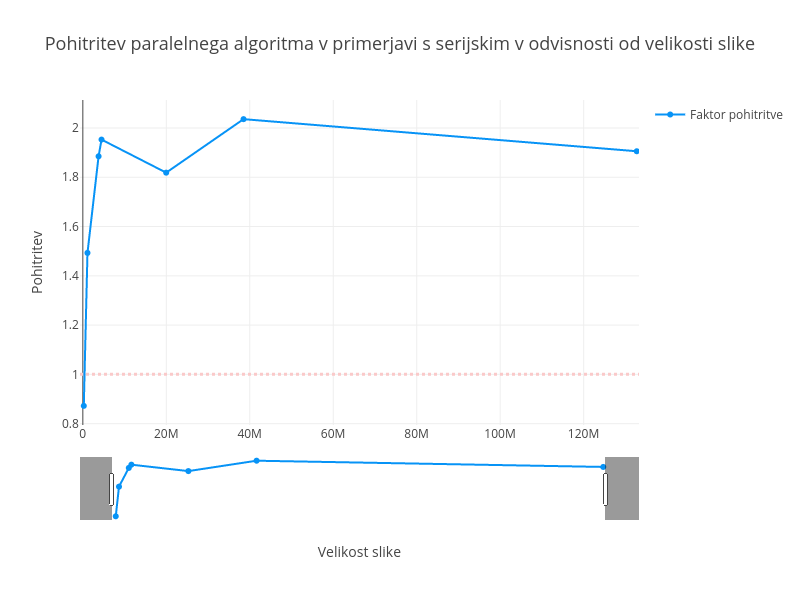
\includegraphics[width=1.2\textwidth]{plot1.png}
\end{center}
\caption{Faktor pohitritve paralelnega algoritma.}
\label{pic1}
\end{figure}

\begin{figure}[htbp]
\begin{center}
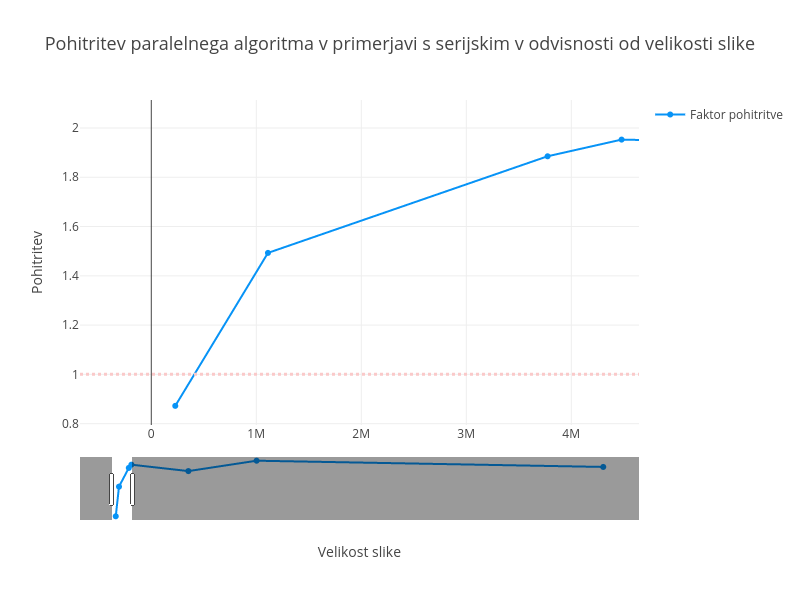
\includegraphics[width=1.2\textwidth]{plot2.png}
\end{center}
\caption{Faktor pohitritve paralelnega algoritma na majhnih slikah.}
\label{pic2}
\end{figure}

\end{document}  




